% !TeX root = book.tex
% !TeX TS-program = pdflatex
% !TeX encoding = UTF-8
% !TeX spellcheck = nl_NL



%% Warn me about obsolete Latex stuff
\RequirePackage[l2tabu, orthodox]{nag}

%% Some credentials about the author
\newcommand{\bookauthor}{Jesse op den Brouw}
\newcommand{\booktitleI}{Elektrische}
\newcommand{\booktitleII}{Netwerken}
\newcommand{\booktitle}{\booktitleI{} \booktitleII}
\newcommand{\booksubtitle}{Een inleiding in de elektrische netwerktheorie}
\newcommand{\bookinstitution}{De Haagse Hogeschool}
\newcommand{\bookedition}{Eerste druk}
\newcommand{\bookversion}{0.1}
\newcommand{\bookkeywords}{elektriciteit elektrische netwerken}
\newcommand{\email}{J.E.J.opdenBrouw@hhs.nl}
%% Nice text on empty pages, or not...
%\newcommand{\thispageintentionallyleftblank}{Deze pagina is opzettelijk leeg gelaten.}
\newcommand{\thispageintentionallyleftblank}{}
%% Include advanced sections
\newcommand{\bookuseadvanded}{\useadvancedtrue}
%%\newcommand{\bookuseadvanded}{\useadvancedfalse}
%% Pick one or none, placed in outer upper corner
\newcommand{\finalconceptdraft}{CONCEPT}
%% Which part to include in the book
\newcommand{\bookpartI}{\usebookpartIfalse}
\newcommand{\bookpartII}{\usebookpartIIfalse}
\newcommand{\bookpartIII}{\usebookpartIIItrue}
\newcommand{\bookasbook}{\usebookasbookfalse}


\input{book_preamble}
%%%%%%%%%%%%%%%%%%%%%%%%%%%%%%%%%%%%%%%%%%%%%%%%%%%%%%%%%%%%%%%%%%%%%
%%
%% TIKZ AND FRIENDS
%%
%%%%%%%%%%%%%%%%%%%%%%%%%%%%%%%%%%%%%%%%%%%%%%%%%%%%%%%%%%%%%%%%%%%%%
\usepackage{calc}
%\usepackage[betterproportions,siunitx]{circuitikz}
\usepackage{circuitikz-dutch}
%\usepackage[betterproportions]{circuitikz}
\usetikzlibrary{bending}
\usetikzlibrary{arrows.meta,arrows}
\usepackage{pgfplots}
\usetikzlibrary{intersections}
\usepgfplotslibrary{units}
\pgfplotsset{compat=1.16}

%\makeatletter
%\usepgflibrary{profiler}
%\pgfprofilenewforenvironment{tikzpicture}
%\pgfprofilenewforenvironment{equation}
%\pgfprofilenewforcommand{\pgfusepath}{1}
%%\pgfprofilenewforcommand{\pgf@circ@drawvoltagegeneric}{}
%\pgfprofilenewforcommand{\pgfnode}{5}
%\pgfprofilenewforcommand{\pgfmathparse}{1}
%\makeatother


% Directory prefix for Gnuplot plots
\tikzset{prefix=gnuplot/}
% Bipoles have the same line witdh as the wires
\ctikzset{bipoles/thickness=1}
% Style for schematics
\tikzset{bookcircuit/.style={line width=1pt,scale=1.25}}

% Get the x and y coordinates of a point
\makeatletter
\newcommand{\gettikzxy}[3]{%
  \tikz@scan@one@point\pgfutil@firstofone#1\relax
  \global\edef#2{\the\pgf@x}%
  \global\edef#3{\the\pgf@y}%
}
\makeatother

% Transform x coordinate to graph coordinate
\makeatletter
\newcommand\transformxdimension[1]{
    \pgfmathparse{((#1/\pgfplots@x@veclength)+\pgfplots@data@scale@trafo@SHIFT@x)/10^\pgfplots@data@scale@trafo@EXPONENT@x}
}
% Transform y coordinate to graph coordinate
\newcommand\transformydimension[1]{
    \pgfmathparse{((#1/\pgfplots@y@veclength)+\pgfplots@data@scale@trafo@SHIFT@y)/10^\pgfplots@data@scale@trafo@EXPONENT@y}
}
\makeatother

%%%\pgfplotsset{xticklabel={$\mathsf{\pgfmathprintnumber{\tick}}$},
%%%             yticklabel={$\mathsf{\pgfmathprintnumber{\tick}}$},
%%%             every axis/.append style={font=\sffamily}
%%%}

%%
%% Dutch inductors are like American inductors, but resistors are european
%%
\ctikzset{inductor = american}
\ctikzset{resistor = european}
%\pgf@circuit@bipole@voltage@straighttrue

\makeatletter

%%
%% Dutch independent current source
%%
%% Extra space for label
%\gdef\pgf@circ@res@cursep{0ex}
%
%%% 4 pt label separation from the arrow
%\ctikzset{bipoles/isource/labelsep/.initial=4}



%%%%%%%%%%%%%%%%%%%%%%%%%%%%%%%%%%%%%%%%%%%%%%%%%%%%%%%%%%%%%%%%%%%%%

%%
%% based on https://tex.stackexchange.com/questions/476045/euler-and-minus-sign
%%
%% Imaginary unit, e, and Euler
\newcommand\imaginaryunit{j}                   % the imaginary unit, i for mathematician and theoretical physicist,
                                               % j for the rest of the world.
\newcommand\imunit{\mathrm{\imaginaryunit}}    % ... in upright math
\newcommand\ce{\mathrm{e}}                     % the constant e, upright of course

\newcommand{\epowre}[1]{\ce^{#1}}              % e to the power of real
\makeatletter
\newcommand{\fiximunit@@}{\if\imaginaryunit j\,\fi}
\newcommand{\epowim}[1]{\ce^{\epowim@#1}}      % e to the power of imaginary
\newcommand{\epowim@}{\@ifnextchar-{\epowim@@}{\epowim@@{\fiximunit@@}}}
\newcommand{\epowim@@}[1]{#1\imunit}
\newcommand{\epowim@@@}{\@ifnextchar-{\epowim@@@@}{+\epowim@@@@{}}}
\newcommand{\epowim@@@@}[1]{#1\imunit}
\newcommand{\epowcom}[2]{\ce^{#1\epowim@@@#2}} % e to the power of complex
\newcommand{\cis}[1]{\cis@#1}                  % cos + imaginary sin
\newcommand{\cis@}{\@ifnextchar-{\cis@@@}{\cis@@}}
\newcommand{\cis@@}[1]{\cos#1 + \imunit\sin#1}
\newcommand{\cis@@@}[2]{\cos#2 - \imunit\sin#2}
%\renewcommand{\Re}{\mathrm{Re}}  % Redefine \Re
%\renewcommand{\Im}{\mathrm{Im}}  % Redefine \Im

\makeatother

\endinput


\begin{document}
\raggedbottom

%%%%%%%%%%%%%%%%%%%%%%%%%%%%%%%%%%%%%%%%%%%%%%%%%%%%%%%%%%%%%%%%%%%%%%%%%%%%%%
%
%  THE FRONTMATTER - title page, preface and table of contents
%
%%%%%%%%%%%%%%%%%%%%%%%%%%%%%%%%%%%%%%%%%%%%%%%%%%%%%%%%%%%%%%%%%%%%%%%%%%%%%%
\frontmatter

%% Pull in the title page, preface and table of contents
%%%%%%%%%%%%%%%%%%%%%%%%%%%%%%%%%%%%%%%%%%%%%%%%%%%%%%%%%%%%%%%%%%%
%%%
%%%       TITLE PAGE
%%%
%%%%%%%%%%%%%%%%%%%%%%%%%%%%%%%%%%%%%%%%%%%%%%%%%%%%%%%%%%%%%%%%%%


%%%%% Make title page
%% Title page defined in preamble
\maketitle

\hspace*{0em}
\vfill
\textcopyright\the\year\ \ \bookauthor, Den Haag\\
Versie: \bookversion\\
Datum: \today

\vspace*{.25cm}
\ifusebookasbook\else
\includegraphics[scale=0.5]{images/HHS_grijs_groen_fc}
\fi

\ifusebookasbook
\vspace*{1cm}
\begin{tabbing}
\hspace{1.2cm}\=\kill
 ISBN: \> 978-XX-XXX-XXXX \\ 
 NUR:  \> 173/959
\end{tabbing}
\fi

\vspace*{2cm}
\includegraphics{images/by-nc-sa_eu.pdf}
\par
{\small%
\booktitle{} van \bookauthor{} is in licentie gegeven volgens
een \href{http://creativecommons.org/licenses/by-nc-sa/3.0/nl/}{Creative Commons
Naamsvermelding-NietCommercieel-GelijkDelen 3.0 Nederland-licentie}.

Suggesties en/of opmerkingen over dit boek kunnen worden gestuurd naar:\\
\href{mailto:\email}{\email}.}
%%%%%%%%%%%%%%%%%%%%%%%%%%%%%%%%%%%%%%%%%%%%%%%%%%%%%%%%%%%%%%%%%%%%%%%%%%%%%%%%%
%%%
%%%   VOORWOORD
%%%
%%%%%%%%%%%%%%%%%%%%%%%%%%%%%%%%%%%%%%%%%%%%%%%%%%%%%%%%%%%%%%%%%%%%%%%%%%%%%


\chapter{Voorwoord}
\label{cha:voorwoord}


\subsubsection*{Leeswijzer}

\subsubsection*{Studiewijzer}
%%%In onderstaande tabel wordt een overzicht gegeven van de stof die een student
%%%bij een eerste introductie onderwezen zou moeten krijgen. Uiteraard is iedereen
%%%vrij om zelf de onderwerpen te kiezen.
%%%
%%%\begin{tabbing}
%%%\hspace{1em}\=\hspace{3cm}\=\kill
%%%\ifusebookpartI
%%%   \> \textbf{Inleiding} \> \\
%%%   \>  Hoofdstuk 1 \> 1.1--1.6, 1.7 (alleen 1.7.1), 1.8--1.12  \\ 
%%%   \>  Hoofdstuk 2 \> 2.1--2.11, 2.13, 2.15 \\ 
%%%   \>  Hoofdstuk 3 \> 3.1--3.6, 3.9, 3.10 \\ 
%%%   \>  Hoofdstuk 4 \> 4.1--4.3 (alleen 4.3.1 en 4.3.2), 4.4--4.6, 4.8--4.10 \\ 
%%%   \>  Hoofdstuk 5 \> 5.1--5.3, 5.6--5.19, 5.21, 5.23 \\ 
%%%   \>  Hoofdstuk 6 \> 6.1--6.3, 6.5, 6.6, 6.8--6.12, 6.15--6.18 \ifusebookpartII \\ \fi
%%%\fi
%%%\ifusebookpartII
%%%   \>              \> \\
%%%   \> \textbf{Geavanceerd 1} \> \\
%%%   \>  Hoofdstuk 7 \> helemaal \\
%%%   \>  Hoofdstuk 8 \> 8.1, 8.3, 8.6 (aanbevolen 8.2, 8.4 en 8.5) \\
%%%   \>  Hoofdstuk 9 \> helemaal \\
%%%   \>  Hoofdstuk 10 \> helemaal \ifusebookpartIII \\ \fi
%%%\fi
%%%\ifusebookpartIII
%%%	\ifusebookpartI\ifusebookpartII\else \\ \fi\fi
%%%   \>              \> \\
%%%   \> \textbf{Geavanceerd 2} \> \\
%%%   \>  Hoofdstuk 11 \> helemaal \\
%%%   \>  Hoofdstuk 12 \> helemaal \\
%%%   \>  Hoofdstuk 13 \> helemaal
%%%\fi
%%%\end{tabbing}


\subsubsection*{Verantwoording inhoud}
%%%\ifusebookasbook
%%%Dit boek voldoet aan acht van de negen punten die opgesomd zijn bij het aandachtsgebied
%%%Digitale techniek in de basis Body of Knowlegde and Skills (BoKS) Elektrotechniek
%%%zoals is vastgelegd door de HBO Engineering. Alleen het onderdeel AD/DA ontbreekt. De
%%%BoKS is te vinden via~\cite{hboengineering2016boks}.
%%%\fi

\subsubsection*{Website}
Op de website \url{http://ds.opdenbrouw.nl} zijn slides, practicumopdrachten
en aanvullende informatie te vinden. De laatste versie van dit boek wordt
hierop gepubliceerd. Er zijn ook voorbeeldprojecten voor de Quartus-software
van Altera te vinden. De projecten kunnen vaak zonder aanpassingen op het
DE0-bordje van Terasic uitgeprobeerd worden.

\subsubsection*{Dankbetuigingen}

%\bigskip%
\hfill \author, \the\year.

%%\input{book_toc.tex}

%%
\mainmatter
%\chapter{Introductie}
\label{cha:introductie}


\section{Spanning en stroom}
De elektrische grootheden spanning en stroom komen voort uit de theorie van de \textsl{elektromagnetische velden}. Een elektromagnetisch veld is een natuurkundig verschijnsel geproduceerd door elektrisch geladen objecten. Het is een van de vier fundamentele krachten in de natuur, naast de zwaartekracht, de zwakke wisselwerking en sterke wisselwerking. Het is lastig om een elektromagnetisch veld voor te stellen, het is immers niet te zien. We kunnen het wel meten met behulp van een \textsl{veldsterktemeter}.

Materie bestaat uit atomen die zijn opgebouwd uit protonen, neutronen en elektronen. Protonen hebben een positieve lading ter grootte van de \textsl{elementaire lading}. Deze lading is gedefinieerd als \SI{1.602176634e-19}{\coulomb} (vanaf 20 mei 2019) en wordt doorgaans aangegeven met de constante $e$ (niet te verwarren met e, het grondtal van de natuurlijke logaritme). Elektronen hebben dezelfde lading maar dan tegengesteld, dus $-e$. Neutronen hebben geen lading. De keuze voor positieve en negatieve lading is ingegeven door het historische feit dat de positieve lading (althans, wat we verstaan onder positieve lading) eerder is ontdekt dan negatieve lading. Pas later werd bekend dat elektriciteit grotendeels wordt veroorzaakt door bewegende elektronen.

Metaalatomen zijn opgelijnd in een zogenoemd kristalrooster. De elektronen in de buitenste schil van een metaalatoom kunnen zich vrijelijk bewegen. Ze springen van de ene atoom naar de andere atoom. Als een elektron migreert naar een atoom, dan wordt dit atoom tijdelijk negatief geladen. Het atoom waar de elektron is weggegaan, is dan positief geladen. Er is een \textsl{gat} ontstaan. Dit ladingsverschil zorgt ervoor dat elektronen zich naar het gat bewegen. Het nettoresultaat van de lading in een metalen geleider is dus 0.

Elektrische spanning is het verschil in \textsl{potentiële elektrische energie} tussen twee punten per eenheid van lading. In het SI-stelsel kan dit worden uitgedrukt in joule per coulomb (\si[per-mode=symbol]{\joule\per\coulomb}), maar spanning heeft een eigen eenheid gekregen: de \textsl{volt}, afgekort tot \si{\volt}. Als symbool voor de elektrische spanning wordt $U$ gebruikt maar in Engelstalige literatuur wordt $V$ gebruikt. Als we een spanningsverschil over een metalen geleider plaatsen, dan geven we de elektronen de mogelijkheid om deze potentiële energie te benutten. Het gevolg is dat de elektronen zich makkelijker kunnen losmaken van de atomen. Omdat positieve en negatieve lading elkaar aantrekken, verplaatsen de elektronen zich naar de positieve spanningspunt. Zodoende vormt zich een \textsl{elektrische stroom}. Er ontstaat dan een tekort aan elektronen aan het negatieve spanningspunt. Om het evenwicht te bewaren, moeten de spanningsbron en de metalen geleider dus een gesloten lus vormen zodat de elektronen vrijelijk kunnen bewegen. We noemen dit een \textsl{stroomkring}. Is de lus niet gesloten, dan ontstaat er geen stroom.

Historisch gezien loopt de stroom van de positieve spanning naar de negatieve spanning, maar \textsl{de elektronenstroom} loopt van de negatieve spanning naar de positieve spanning. Elektrische stroom is de hoeveelheid verplaatste lading per tijdseenheid, en wordt uitgedrukt in ampère, afgekort tot \si{\ampere}. Als symbool wordt $I$ gebruikt. Niet de lading maar de elektrische stroom is een van de zeven grondgrootheden van het SI-stelsel. Lading is dus uit te drukken als stroom keer tijd, oftewel \si{\ampere\second}. We zouden verwachten dat de elektronen zich zeer snel verplaatsen in de geleider. Een elektrisch lichtpunt gaat immers gelijk branden als we de schakelaar omhalen. Toch is dat niet zo. De \textsl{driftsnelheid} van elektronen is klein: ongeveer \SI[per-mode=symbol]{0,1}{\milli\meter\per\second}. Waarom een lichtpunt gelijk gaat branden komt omdat de (langzaam) bewegende elektronen tegen elkaar botsen en zo hun \textsl{impuls} doorgeven. Het is te vergelijken met een stilstaande rij, tegen elkaar geplaatste, biljartballen. Als er een biljartbal tegen het uiteinde van de rij botst, zal aan bij het uiteinde van de rij een biljartbal snelheid krijgen. De tussenliggende biljartballen verplaatsen zich niet, ze geven alleen de impuls door. 


%dus uitgedrukt in \si{\coulomb\per\second}. 


%Elektrische stroom is beweging van elektrische lading. De elektrische stroom die in een metalen geleider vloeit, zoals koper en aluminium, bestaat uit verplaatsende elektronen. De protonen en neutronen in de geleider verplaatsen zich niet. Als op een metalen geleider een spanning (spanningsverschil) wordt aangebracht, bewegen de elektronen zich naar de positieve spanning.  





\subsection{Definitie van stroom}
De elektrische stroom is een van de zeven basisgrootheden van het SI-stelsel. Een elektrische stroom is niets anders dan een hoeveelheid lading die per seconde door het oppervlakte van de dwarsdoorsnede van een geleider vloeit:
%
\begin{equation}
\SI{1}{\ampere} = \SI[per-mode=fraction]{1}{\coulomb\per\second}
\end{equation} 

\subsubsection*{Tot en met 19 mei 2019}
In twee rechte geleiders loopt een stroom van \SI{1}{\ampere} als de twee geleiders van oneindige lengte en verwaarloosbare diameter, geplaatst in vacuüm op een afstand van \SI{1}{\meter}, een kracht op elkaar uitoefenen van \SI[per-mode=symbol]{2e-7}{\newton\per\meter}.

\subsubsection*{Vanaf 20 mei 2019}
Vanaf deze datum is de elementaire lading vastgesteld op \SI{1.602176634e-19}{\coulomb}. De stroom is gedefinieerd op basis van de elementaire lading. Dit zorgt ook voor de herdefinitie van de coulomb. In een geleider loopt een stroom van \SI{1}{\ampere} als per seconde een lading $\frac{1}{\num{1.602176634e-19}}\si{\coulomb}$ passeert.

\section{Meten van spanning en stroom}
Om een spanning tussen twee punten te meten, gebruiken we een \textsl{spanningsmeter}. De spanningsmeter heeft twee ingangen, de `+'-ingang en de `$-$'-ingang. Als de spanning op de `+'-ingang groter is dan de spanning op de `$-$'-ingang, dan geeft de meter een positieve spanning aan. Omgekeerd heeft de meter een negatieve spanning aan.

\begin{infobox}[Naming and shaming\ldots]
Een spanningsmeter wordt in de volksmond ook wel een \textsl{voltmeter} genoemd. Dit is echter niet juist. Er wordt een grootheid gemeten, spanning, die wordt uitgedrukt in volt. Evenzo wordt voor het meten van een stroom een stroommeter gebruikt, in de volksmond een \textsl{ampèremeter} genoemd. Ook dit is niet juist. Een stroommeter meet de grootheid stoom en die wordt uitgedrukt in ampère. En zo kunnen we doorgaan: een vermogensmeter en geen \textsl{wattmeter}, een frequentiemeter en geen \textsl{hertzmeter}, een thermometer en geen \textsl{kelvinmeter} (of graden-celsiusmeter)

In Amerika wordt echter wel de termen \textsl{voltmeter} en \textsl{ammeter} gebruikt.

Soms wordt voor spanning het woord \textsl{voltage}, voor stroom \textsl{ampèrage} en voor vermogen \textsl{wattage} gebruikt. Allemaal onjuist, hoewel voltage nog wel enigszins kan.
\end{infobox}



\begin{table}[!ht]
\centering
\caption{Soortelijke weerstand $\rho$ in \si{\ohm\meter} bij \SI{20}{\celsius} en temperatuurcoëfficiënt $\alpha$ in \si{\per\kelvin} van enkele materialen.}
\begin{tabular}{lSS}
\toprule
Materiaal & {Soortelijke weerstand} & {Temp. coëfficiënt} \\
\midrule
Zilver & 1.59e-8 & 0.0041 \\
Koper & 1.75e-8 & 0.0039 \\
Goud & 2.20e-8 & 0.0036 \\
Aluminium & 2.65e-8 & 0.0043 \\ 
%&&\\
%Glas & 1e12 & {$-$} \\
\bottomrule
\end{tabular}
\end{table}

%\section{Opgaven}
%\input{book_chap01_ques}
\chapter{Gelijkstroomtheorie}
In dit hoofdstuk behandelen we de gelijkstroomtheorie. Nu suggereert het woord
gelijkstroomtheorie dat de theorie alleen de stromen betreft. Dat is echter niet
het geval; het betreft ook de spanningen. We kunnen dus net zo goed spreken over
gelijkspanningstheorie. De keuze voor gelijkstroomtheorie is ingegeven doordat de
grootheid elektrische stroom als een van de zeven grondgrootheden in
het SI-stelsel is gekozen.

In de gelijkstroomtheorie veronderstellen we dat de alle spanningen en stromen
een constante waarden hebben over de tijd. De spanningen en stromen vari\"eren
dus niet als functie van de tijd\footnote{Formeel gezien is een spanning of stroom
die niet van polariteit veranderd ook een gelijkspanning of gelijkstroom. We
veronderstellen hier echter dat de spanningen en stromen constant zijn.}.
 Ze kunnen zowel positief als negatief zijn,
of nul.

In de gelijkstroomtheorie hebben we drie componenten: de ideale
spanningsbron, de ideale stroombron en de ideale weerstand. De
symbolen die gebruikt worden in schakelschema's zijn te zien in
figuur~\ref{fig:symbolenbronnenenweerstand}. Een
ideale spanningsbron levert een constante spanning ongeacht de
stroom die de bron levert. Een ideale stroombron levert een
constante stroom ongeacht de spanning die over de bron staat.
Een ideale weerstand heeft een constante waarde ongeacht de
spanning over en de stroom door de weerstand. Verder merken
we op dat de ideale spanningsbron een interne weerstand heeft
van 0 Ohm. De interne weerstand van de ideale stroombron is
oneindig.

\begin{figure}[!ht]
\centering
\begin{subfigure}{0.30\textwidth}
\centering
\begin{tikzpicture}[line width=1pt]
\draw (0,0) to [V<=$U$] (0,2);
\end{tikzpicture}
\caption{Symbool ideale spanningsbron.}
\label{fig:gelidealespanningsbron}
\end{subfigure}
\begin{subfigure}{0.30\textwidth}
\centering
\begin{tikzpicture}[line width=1pt]
\draw (0,0) to [I, l=$I$, n=I, inner sep=5pt] (0,2);
%\node[left=2pt] at (I.n) {$I$};
\end{tikzpicture}
\caption{Symbool ideale stroombron.}
\end{subfigure}
\begin{subfigure}{0.30\textwidth}
\centering
\begin{tikzpicture}[line width=1pt]
\draw (0,0) to [R, l=$R$] (0,2);
\end{tikzpicture}
\caption{Symbool ideale\\ weerstand.}
\end{subfigure}
%\caption{blabla \protect\subref{fig:gelidealespanningsbron} blabla}
\caption{Symbolen voor de ideale spanningsbron, de ideale stroombron en de ideale weerstand.}
\label{fig:symbolenbronnenenweerstand}
\end{figure}

Voor het aangeven van spanningen gebruiken we de hoofdletter $U$. In Engelstalige boeken
wordt de hoofdletter $V$ gebruikt. Spanning worden uitgedrukt in V (volt). Stromen worden
aangegeven met een hoofdletter $I$ en worden uitgedrukt in A (amp\`ere). Weerstanden
geven we aan met de hoofdletter $R$ (van het Engelse woord \textsl{resistor}) en worden
uitgedrukt in $\Omega$ (ohm).

We kunnen de waarden van spanningen, stromen en weerstanden ook uitdrukken door er een
letter voor te zetten, de zogenoemde SI-voorvoegsels: mV (millivolt), mA (milliamp\`ere),
$\muup$A (microamp\`ere), k$\Omega$ (kilo-ohm), M$\Omega$ (megaohm).

\section{Stroomwet van Kirchhof}
De stroomwet van Kirchhoff zegt dat alle stromen naar een knooppunt toe opgeteld 0 zijn.
Er kan dus geen stroom bijkomen of verloren gaan. In formulevorm:
\begin{equation}
I_1 + I_2 + \cdots + I_n = 0
\end{equation}
Ander gezegd: de totale stroom die naar een knooppunt toevloeit is even groot als de
totale stroom die van het knooppunt wegvloeit. In figuur~\ref{fig:gelstroomwetKirchhoff}
is de stroomwet uitgebeeld.

\begin{figure}[!ht]
\centering
\begin{tikzpicture}[line width=1pt]
\draw (-2,1) to [short, i=$I_1$, -*] (0,0);
\draw (-1.5,-1.5) to [short, i=$I_2$, -*] (0,0);
\draw (2,0.5) to [short, i=$I_3$, -*] (0,0);
\draw (1,-1.5) to [short, i=$I_4$, -*] (0,0);
\end{tikzpicture}
\caption{De stroomwet van Kirchhoff: de stromen naar een knooppunt toe zijn opgeteld 0.}
\label{fig:gelstroomwetKirchhoff}
\end{figure}

In het geval dat een knooppunt slechts twee aansluitingen heeft, is de ingaande stroom even groot als de
uitgaande stroom. Zie figuur~\ref{fig:gelingaandeIisuitgaandeI}.

\begin{figure}[!ht]
\centering
\begin{tikzpicture}[line width=1pt]
\draw (0,0) to [short, i>=$I_1$, -*] ++(3,0) node[above,yshift=1cm] {$I_1=I_2$} to [short, i>=$I_2$] ++(3,0);
\end{tikzpicture}
\caption{De ingaande stroom is even groot als de uitgaande stroom.}
\label{fig:gelingaandeIisuitgaandeI}
\end{figure}



\section{De spanningswet van Kirchhof}
De spanningswet van Kirchhoff zegt dat alle spanningen in een gesloten kring opgeteld~0
zijn. Er kan dus geen spanning bijkomen of verloren gaan. In formulevorm:
\begin{equation}
U_1 + U_2 + \cdots + U_n = 0
\end{equation}

Anders gezegd: de totale spanning rechtsom opgeteld, is even groot als de totale spanning linksom opgeteld. In figuur~\ref{fig:spanningswetKirchhoff} is de spanningswet uitgebeeld.

\begin{figure}[!ht]
\centering
\begin{tikzpicture}[line width=1pt]
\draw (0.0,0.0)  node[left] {$+$} to [short, o-] ++(0.0,1.0) to [short, -o]  node[above] {$-$} ++(1.0,0.0)
      to [open,l=$U_2$,above] ++(0.5,0.0) node[above] {$+$} to [short, o-] ++(1.0,0.0) to [short, -o] node[right] {$-$} ++(0.0,-1.0)
      to [open,l=$U_3$,inner sep=8pt] ++(0.0,-0.5) node[right] {$+$} to [short, o-] ++(0.0,-1.0) to [short, -o] node[below] {$-$} ++(-1.0,0.0)
      to [open,l=$U_4$,above] ++(-0.5,0.0) node[below] {$+$} to [short, o-] ++(-1.0,0.0) to [short, -o] node[left] {$-$} ++(0.0,1.0)
      to [open,l=$U_1$,inner sep=8pt] ++(0.0,0.5);
\end{tikzpicture}
\caption{De spanningswet van Kirchhoff: alle spanningen in een kring zijn opgeteld 0.}
\label{fig:spanningswetKirchhoff}
\end{figure}

Als een verbinding zich vertakt over twee parallel geschakelde netwerkelementen is de spanning over
de netwerkelementen gelijk. Dit is te zien in figuur~\ref{fig:gelspanningengelijk}.

\begin{figure}[!ht]
\centering
\begin{tikzpicture}[line width=1pt]
\draw (0,0) to[short,-*]++(1,0) to[short] ++(0,0.5) to[short,-o,] node[above] {$+$} ++(1,0) to[open, l=$U_1$,above] ++(1,0) node[above] {$-$} to[short, o-] ++(1,0) to[short,-*] ++(0,-.5) to[short] ++(1,0) to[open] ++(-1,0) to[short] ++(0,-0.5) to[short,-o] node[below] {$-$} ++(-1,0) to [open,l=$U_2$,-o] ++(-1,0) node[below] {$+$} to [short] ++(-1,0) to [short] ++(0,0.5);
\draw (0,1) node {$U_1=U_2$};
\end{tikzpicture}
\caption{De spanningen over twee parallel geschakelde elementen zijn gelijk.}
\label{fig:gelspanningengelijk}
\end{figure}




\section{De wet van Ohm}
De verhouding tussen de spanning over een weerstand en de stroom door de weerstand is constant
en wordt de wet van Ohm genoemd. De wet wordt meestal geschreven als:
\begin{equation}
U=I\cdot R
\end{equation}
%
Gegeven een bepaalde spanning en stroom, dan kan de weerstandswaarde berekend worden met:
%
\begin{equation}
R = \dfrac{U}{I}
\end{equation}
%
In figuur~\ref{fig:geldewetvanohm} is de wet van Ohm uitgebeeld. Aan de spanningbron $U$ wordt
een weerstand $R$ geplaatst. We spreken dan dat de spanningsbron wordt belast. Ook hier geldt de
spanningswet van Kirchhoff: de spanning $U$ van de bron is gelijk aan de spanning $U_R$ over de
weerstand. Bij de gegeven richting van de stroom $I$ geldt dat het potentiaal bij de `$+$' groter
is dan het potentiaal bij de `$-$'.

\begin{figure}[!ht]
\centering
\begin{tikzpicture}[line width=1pt]
\draw (0,0) to [V<=$U$] ++(0,2) to [short, i=$I$] ++(2.5,0) to [R=$R$, v=$U_R$] ++(0,-2) to [short,-.] (0,0)
;
%%%\draw (-2,0) to[short, i=$I$] (0,0);
%%%\draw (0,0) to[R=$R$, v_>=$U$] (2,0);
\end{tikzpicture}
\caption{De spanning over en stroom door een weerstand is constant.}
\label{fig:geldewetvanohm}
\end{figure}

\section{Serieschakeling van weerstanden}
In figuur~\ref{fig:gelserieschakelingweerstanden} is een schakeling te zien waarbij de weerstanden
in serie geschakeld zijn en gevoed worden door een spanningsbron. De spanningsbron levert een stroom
$I$ waardoor de spanningsbron een bepaalde weerstand ondervindt. We noemen deze weerstand $R_s$.

\begin{figure}[!ht]
\centering
\begin{tikzpicture}[line width=1pt]
\draw (0,0) to [V<=$U$] ++ (0,2) to [short, i=$I$] ++(2,0)
            to [R, l=$R_1$,v=$U_1$] ++(2,0) to [R, l=$R_2$, v=$U_2$] ++(2,0)
            coordinate (A);
\draw[dotted] (A) --  ++(1,0) coordinate (B);
\draw (B) to [R,l=$R_n$,v=$U_n$] ++(2,0) to [short] ++(0.5,0) to [short] ++(0,-2) to [short,-.] (0,0);
\end{tikzpicture}
\caption{Serieschakeling van weerstanden.}
\label{fig:gelserieschakelingweerstanden}
\end{figure}

Vanuit de spanningswet van Kirchhoff volgt dat:
%
\begin{equation}
U=U_1+U_2+\cdots+U_n
\end{equation}
%
Vanuit stroomwet van Kirchhoff volgt dat:
%
\begin{equation}
I = I_1 = I_2 = \cdots = I_n
\end{equation}
%
De stroom die de bron levert is dus even groot als de stromen door de weerstanden.
De bron met spanning $U$ levert een stroom $I$ zodanig dat:
%
\begin{equation}
U=I\cdot R_s
\end{equation}
%
Dus volgt dat:
%
\begin{equation}
I\cdot R_s = I\cdot R_1+I\cdot R_2+\cdots+I\cdot R_n
\end{equation}
%
We schappen aan beide kanten $I$ zodat volgt dat:
%
\begin{equation}
R_s = R_1 + R_2 + \cdots R_n
\end{equation}
%
Hierbij is $R_s$ de vervangingswaarde van de in serie geschakelde weerstanden.


\section{Parallelschakeling van weerstanden}
In figuur~\ref{fig:gelparalledschakelingweerstanden} is een parallelschakeling van een
aantal weerstanden te zien. De schakeling wordt gevoed door de spanningsbron $U$. Als
gevolg van de weerstanden zal de bron een bepaalde stroom leveren. Hierdoor ondervindt
de spanningsbron een bepaalde weerstand. Deze weerstand noemen we $R_p$.

\begin{figure}[!ht]
\centering
\begin{tikzpicture}[line width=1pt]
%% Draw voltage source, wire with current I, resistor R1 and back to minus of voltage source
\draw (0,0) to [V<=$U$] ++ (0,2) to [short] ++(0,0.25) to [short,i=$I$,-*] ++(3,0) coordinate (A) to [short] ++(0,-0.25) to[R=$R_1$,-*,i>^=\small $I_1$,v=\small $U_1$] ++(0,-2) to [short,-.] (0,0);
%% Draw resistor R2 and wire to minus of resistor R1
\draw (A) to[short,-*] ++(2,0) coordinate (B) to [short] ++(0,-0.25) to [R=$R_2$,-*,i>^=\small $I_2$, v=\small $U_2$] ++(0,-2) to [short] ++(-2,0);
%% Draw short heading to Rk
\draw (B) to[short] ++(0.75,0) coordinate (C);
%% Draw dotted wire
\draw[dotted] (C) -- ++(1,0) coordinate (D);  
%% Draw Rk
\draw (D) to [short] ++(0.75,0) to [short] ++(0,-0.25) to [R=$R_n$,i>^=\small $I_n$, v=\small $U_n$ ] ++(0,-2) to [short] ++(-0.75,0) coordinate (E);
%% Draw dotted wire
\draw[dotted] (E) -- ++(-1,0) coordinate (F);
%% Draw wire to minus of R2
\draw (F) to [short] ++(-0.75,0);
\end{tikzpicture}
\caption{Parallelschakeling van weerstanden.}
\label{fig:gelparalledschakelingweerstanden}
\end{figure}

Vanuit de spanningswet van Kirchhoff vinden we dat:
%
\begin{equation}
U = U_1 = U_2 = \cdots = U_n
\end{equation}
%
De spanningen over de weerstanden zijn even groot als de bronspanning.
Vanuit de stroomwet van Kirchhoff vinden we dat:
%
\begin{equation}
I = I_1 + I_2 + \cdots + I_n
\end{equation}
%
We kunnen de stroomwet ook formuleren als:
%
\begin{equation}
\dfrac{U}{R_p} = \dfrac{U}{R_1} + \dfrac{U}{R_2} + \cdots + \dfrac{U}{R_n}
\end{equation}
%
We schrappen aan beide zijden van de vergelijking de spanning $U$ zodat we krijgen dat:
%
%De vervangingswaarde voor de parallelschakeling van een aantal weerstanden is te berekenen met:
\begin{equation}
\dfrac{1}{R_p} = \dfrac{1}{R_1} + \dfrac{1}{R_2} + \cdots + \dfrac{1}{R_n}
\end{equation}
%
Hierin is $R_p$ de vervangingswaarde van de parallel geschakelde weerstanden.
Voor twee parallel geschakelde weerstanden geldt dat:
\begin{equation}
\dfrac{1}{R_p} = \dfrac{1}{R_1} + \dfrac{1}{R_2}
\end{equation}
%
Dit kan worden omgewerkt tot:
\begin{equation}
R_p = \dfrac{R_1\cdot R_2}{R_1+R_2}
\end{equation}


\section{Spanningsdeling}
In figuur~\ref{fig:gelspanningsdeling} is een schema te zien van een bron met twee in
serie geschakelde weerstanden. De spanning $U$ zal zich in een bepaalde verhouding
verdelen over de twee weerstanden. Er is sprake van spanningsdeling.

\begin{figure}[!ht]
\centering
\begin{tikzpicture}[line width=1pt]
\draw (0,0) to [V<=$U$] ++ (0,2) to [short, i=$I$] ++(1.5,0)
            to [R, l=$R_1$,v=$U_1$] ++(2,0) to [R, l=$R_2$, v=$U_2$] ++(2,0)
            to [short] ++(0.5,0) to [short] ++(0,-2) to [short,-.] (0,0);
\end{tikzpicture}
\caption{Schema voor spanningsdeling.}
\label{fig:gelspanningsdeling}
\end{figure}

De stroom $I$ kunnen we berekenen met:
%
\begin{equation}
I = \dfrac{U}{R_!+R_2}
\end{equation} 
%
Voor de spanningen $U_1$ en $U_2$ kunnen we schrijven dat:
%
\begin{equation}
U_1 = I\cdot R_1 = \dfrac{R_1}{R_1+R_2}\cdot U \qquad\text{en}\qquad U_2 = I\cdot R_2 = \dfrac{R_2}{R_1+R_2}\cdot U
\end{equation}


\section{Stroomdeling}
In figuur~\ref{fig:gelstroomdeling} is een schema te zien van een bron met twee parallel
geschakelde weerstanden. De stroom $I$ zal zich in een bepaalde verhouding
verdelen over de twee weerstanden. Er is sprake van stroomdeling.

\begin{figure}[!ht]
\centering
\begin{tikzpicture}[line width=1pt]
%% Draw voltage source, wire with current I, resistor R1 and back to minus of voltage source
\draw (0,0) to [V<=$U$] ++ (0,2) to [short] ++(0,0.25) to [short,i=$I$,-*] ++(3,0) coordinate (A) to [short] ++(0,-0.25) to[R=$R_1$,-*,i>^=\small $I_1$,v=\small $U_1$] ++(0,-2) to [short,-.] (0,0);
%% Draw resistor R2 and wire to minus of resistor R1
\draw (A) to[short] ++(2,0) coordinate (B) to [short] ++(0,-0.25) to [R=$R_2$,i>^=\small $I_2$, v=\small $U_2$] ++(0,-2) to [short] ++(-2,0);
\end{tikzpicture}
\caption{Schema voor stroomdeling.}
\label{fig:gelstroomdeling}
\end{figure}

De spanning $U$ kunnen kunnen we berekenen met:
%
\begin{equation}
U = I\cdot\dfrac{R_1\cdot R_2}{R_1+R_2}
\end{equation}
%
Natuurlijk geldt de stroomwet van Kirchhoff:
%
\begin{equation}
I = I_1 + I_2 = \dfrac{U}{R_1} + \dfrac{U}{R_2}
\end{equation}
%
Voor $I_1$ geldt dan:
%
\begin{equation}
I_1 = \dfrac{U}{R_1} = \dfrac{R_1\cdot R_2}{R_1+R_2}\cdot \dfrac{1}{R_1}\cdot I = \dfrac{R_2}{R_!+R_2}\cdot I
\end{equation}
%
Op vergelijkbare wijze vinden we voor $I_2$:
%
\begin{equation}
I_2 = \dfrac{U}{R_2} = \dfrac{R_1\cdot R_2}{R_1+R_2}\cdot \dfrac{1}{R_2}\cdot I = \dfrac{R_1}{R_!+R_2}\cdot I
\end{equation}


\section{De niet-ideale spanningsbron}
In de praktijk hebben we te maken met niet-ideale spanningsbronnen. We kunnen zo'n bron
weergeven met een ideale spanningsbron in serie met een ideale weerstand. De ideale
weerstand wordt de \textsl{inwendige weerstand} genoemd. Dit is te zien in
\index{inwendige weerstand}
figuur~\ref{fig:gelnisopenkort}.

\begin{figure}[!ht]
\begin{subfigure}{0.5\textwidth}
\centering
\begin{tikzpicture}[line width=1pt]
\draw (0,0) to [V<=$U$] ++(0,2) to [R=$R_i$,-*] coordinate (A) ++(2.5,0) node[right] {$+$} to [open] ++(0,-2) coordinate (B) node[right] {$-$} to [short,*-.] (0,0);
\draw ($(A)!0.5!(B)$) node[right] {$U_o$};
\end{tikzpicture}
\caption{}
\label{fig:gelnisopen}
\end{subfigure}%
\begin{subfigure}{0.5\textwidth}
\centering
\begin{tikzpicture}[line width=1pt]
\draw (0,0) to [V<=$U$] ++(0,2) to [R=$R_i$,-*] ++(2.5,0) to [short, i=$I_k$] ++(0,-2) to [short,*-.] (0,0);
\end{tikzpicture}
\caption{}
\label{fig:gelniskort}
\end{subfigure}
\caption{Niet-ideale spanningsbron: \subref{fig:gelnisopen} onbelast, \subref{fig:gelniskort} kortgesloten.}
\label{fig:gelnisopenkort}
\end{figure}

In figuur~\ref{fig:gelnisopen} is te zien dat de niet-ideale spanningsbron onbelast is.
De spanning $U_o$ is even groot als de bronspanning $U$. Er loopt immers geen stroom zodat
er geen spanningsval over de inwendige weerstand staat. Deze spanning wordt de \textsl{open
klemspanning} genoemd. In figuur~\ref{fig:gelniskort} is
\index{open klemspanning}
de niet-ideale spanningsbron kortgesloten. Over de inwendige weerstand staat nu de volledige
bronspanning. Er loopt dan een zekere \textsl{kortsluitstroom} $I_k$. We kunnen de inwendige
\index{kortsluitstroom}
weerstand berekenen door de uitgangsspanning $U_o$ te delen door de kortsluitstroom $I_k$.

Voor een goede spanningsbron moet de inwendige weerstand klein zijn. Praktische waarden van
de inwendige weerstanden liggen tussen de enkele tientallen m$\Omega$ tot enkele~$\Omega$.
Zo kan een autoaccu met een spanning van 12 V stromen van meer dan 100 A leveren. Het is dan
ook niet aan te bevelen om dergelijke kortsluitstromen te meten. De inwendige weerstand
van eenvoudige batterijen ligt in de orde van enkele $\Omega$. Een laboratoriumvoeding moet
natuurlijk ook een lage inwendige weerstand hebben om de uitgangsspanning zo constant
mogelijk te houden. Veelal is de voeding beschermd tegen kortsluiting en wordt de
kortsluitstroom begrensd.


\section{De niet-ideale stroombron}
In de praktijk hebben we ook te maken met niet-ideale stroombronnen. De niet-ideale
stroombron is te modelleren als een ideale stroombron parallel geschakeld aan een ideale
weerstand. Ook deze weerstand wordt de inwendige weerstand genoemd. Dit is te zien in
figuur~\ref{fig:gelnissopenkort}.

\begin{figure}[!ht]
\begin{subfigure}{0.5\textwidth}
\centering
\begin{tikzpicture}[line width=1pt]
\draw (0,0) to [I, l=$I$, inner sep=5pt] ++(0,2) to [short] ++(1,0) coordinate (A) to [R=$R_i$,*-*]  ++(0,-2) coordinate (B) to [short,-.] (0,0) (A) to [short, -*] ++(1,0) node[right] {$+$} (B) to [short, -*] ++(1,0) node[right] {$-$}; 
\draw ($(A)!0.5!(B)$) node[right,xshift=1cm] {$U_o$};
\end{tikzpicture}
\caption{}
\label{fig:gelnissopen}
\end{subfigure}%
\begin{subfigure}{0.5\textwidth}
\centering
\begin{tikzpicture}[line width=1pt]
\draw (0,0) to [I, l=$I$, inner sep=5pt] ++(0,2) to [short] ++(1,0) coordinate (A) to [R=$R_i$,*-*]  ++(0,-2) coordinate (B) to [short,-.] (0,0) (A) to [short, -*] ++(1,0) to [short, i=$I_k$, -*] ++(0,-2) to [short] (B) ; 
\end{tikzpicture}
\caption{}
\label{fig:gelnisskort}
\end{subfigure}
\caption{Niet-ideale stroombron: \subref{fig:gelnissopen} onbelast, \subref{fig:gelnisskort} kortgesloten.}
\label{fig:gelnissopenkort}
\end{figure}

In figuur~\ref{fig:gelnissopen} is de niet-ideale stroombron onbelast. De stroom $I$
loopt nu door de inwendige weerstand. Hierdoor zal over de bron een bepaalde spanning aanwezig
zijn. We noemen die spanning de open klemspanning. In figuur~\ref{fig:gelnisskort} is de bron
kortgesloten. De stroom $I$ loopt nu volledig door de kortsluiting. We noemen de stroom de
kortsluitstroom. We kunnen de inwendige
weerstand berekenen door de uitgangsspanning $U_o$ te delen door de kortsluitstroom $I_k$.

Voor een goede stroombron moet de inwendige weerstand zo groot mogelijk zijn. Praktische
waarden voor $R_i$ liggen tussen enkele honderden k$\Omega$ tot vele M$\Omega$. Aan
figuur~\ref{fig:gelnissopen} kunnen we nog iets ontdekken. De uitgangsspanning in onbelaste
toestand zal zeer groot zijn. We kunnen nu inzien dat een stroombron dus nooit onbelast gelaten
mag worden. Een laboratoriumvoeding zal de uitgangsspanning in onbelaste toestand begrenzen.

\section{Vermogen ontwikkeld in een weerstand}
Een weerstand waar een spanning over staat en een stroom door loopt dissipeert energie. Dit is weergegeven in
figuur~\ref{fig:gelvermogensdissipatie}. Dat een weerstand energie dissipeert kunnen we merken doordat de
weerstand warm wordt.
Het \textsl{vermogen} dat ontwikkeld wordt in een weerstand is het product van de spanning over
\index{vermogen}
en de stroom door de weerstand:
%
\begin{equation}
P = U\cdot I 
\end{equation}

\begin{figure}[!ht]
\centering
\begin{tikzpicture}[line width=1pt]
\draw (0,0) to [V<=$U$] ++(0,2) to [short, i=$I$] ++(2.5,0) to [R,l_=$R$,n=R] ++(0,-2) to [short,-.] (0,0);
\draw[decorate, decoration={snake, segment length=5pt, amplitude=1pt},->stealth'] (R) ++(0.2,0.2) -> ++(2,0.2);
 \draw[decorate, decoration={snake, segment length=5pt, amplitude=1pt},->stealth'] (R) ++(0.2,0.0) -> ++(2,0.0) node[right] {W};
\draw[decorate, decoration={snake, segment length=5pt, amplitude=1pt},->stealth'] (R) ++(0.2,-0.2) -> ++(2,-0.2); \end{tikzpicture}
\caption{De weerstand dissipeert warmte.}
\label{fig:gelvermogensdissipatie}
\end{figure}


Vermogen wordt uitgedrukt in W (watt). Aangezien we voor $U$ ook kunnen schrijven $U=I\cdot R$
kunnen we ook stellen dat:
\begin{equation}
P = I^2\cdot R
\end{equation}
Verder kunnen we voor $I$ schrijven dat $I=\dfrac{U}{R}$ zodat we kunnen stellen dat:
\begin{equation}
P = \dfrac{U^2}{R}
\end{equation}
%
De eenheid W (watt) kan ook geschreven worden als J/s (joules per seconde) en dat geeft precies
aan wat het vermogen inhoudt: energieafgifte per seconde. Willen we de totale energieafgifte
over een bepaalde tijd $t$ berekenen dan moeten we het vermogen vermenigvuldigen met de tijd:
%
\begin{equation}
W = P\cdot t
\end{equation}
%
De variabele $W$ staat voor het Engelse woord \textsl{Work}. Een veel gebruikte eenheid van energie
is de kWh (kilowattuur). Dit komt overeen met de energie
als een component een vermogen van 1000 W een uur lang dissipeert. De hoeveelheid energie is:
%
\begin{equation}
1\ \mathrm{kWh} = 1000\ \mathrm{W} \times 1\ \mathrm{uur} = 1000\ \dfrac{\mathrm{J}}{\mathrm{s}} \times 3600\ \mathrm{s} = 3.600.000\ \mathrm{J} = 3,6\ \mathrm{MJ}
\end{equation}

%%%De spanning over een spoel kan berekend worden met:
%%%\begin{equation}
%%%U = L\dfrac{\text{d}i}{\text{d}t}
%%%\end{equation}
%%%Hierin is $L$ de zelfinductie van de spoel. Bij een sinusvormige spanning met hoekfrequentie
%%%$\omega$ kunnen we dus schrijven:
%%%\begin{equation}
%%%U = L\dfrac{\text{d}\, i \sin \omega t}{\text{d}t} = \omega L i\cos \omega t
%%%\end{equation}
%%%De amplitude van de spanning is dus afhankelijk van de hoekfrequentie $\omega$.
%%%
%%%De spanning over een condensator kan berekend worden met:
%%%\begin{equation}
%%%U = \dfrac{1}{C}\int i\,\text{d}t 
%%%\end{equation}
%%%
%%%Hierin is $C$ de capaciteit van de condensator. Bij een sinusvormige spanning met hoekfrequentie
%%%$\omega$ kunnen we schrijven:
%%%\begin{equation}
%%%U = \dfrac{1}{C}\int i\sin \omega t\,\text{d}t = -\dfrac{i}{\omega C} \cos \omega t
%%%\end{equation}


\section{Maximale vermogensoverdracht}
In figuur~\ref{fig:maximalevermogensoverdracht} is te zien dat een niet-ideale
spanningsbron met spanning $U$ en inwendige weerstand $R_i$ is verbonden met
een uitwendige weerstand $R_u$. We willen graag maximale vermogensoverdracht
vanuit de bron in $R_u$.

\begin{figure}[!ht]
\centering
\begin{circuitikz}[line width=1pt]
\draw (0,0) to[V<=$U$] ++(0,2) to[R=$R_i$, -*] ++(2,0) to[short, i=$I$] ++(1,0) to[R=$R_u$] ++(0,-2) to[short, -*] ++(-1,0) to[short,-.] (0,0);
\end{circuitikz}
\captionsetup{width=.9\linewidth}
\caption{Een niet-ideale spanningsbron met inwendige weerstand wordt belast met een uitwendige weerstand.}
\label{fig:maximalevermogensoverdracht}
\end{figure}

De stroom die de bron produceert is:
%
\begin{equation}
I = \dfrac{U}{R_i + R_u}
\end{equation}
%
Het vermogen dat in de uitwendige weerstand wordt gedissipeerd is:
%
\begin{equation}
\label{equ:dissipatedru}
P_{Ru} = I^2R_u = \left(\dfrac{U}{R_i+R_u}\right)^2 R_u
       = \dfrac{R_u}{(R_i+R_u)^2}\: U^2
\end{equation}
%
We kunnen inzien dat als $R_u$ klein is de stroom groot zal zijn maar het vermogen in $R_u$ is
dan klein. Als $R_u$ groot is dan zal de stroom klein zijn en ook dan is het
vermogen in $R_u$ klein. Ergens daartussen ligt een optimum waarbij het meeste vermogen
wordt overgedragen in de uitwendige weerstand. Hiertoe differenti\"eren we de vergelijking
\eqref{equ:dissipatedru} naar $R_u$:
%
\begin{equation}
\setlength{\jot}{10pt}
\begin{split}
\dfrac{\text{d}P_{Ru}}{\text{d}R_u} &= U^2\dfrac{(R_i+R_u)^2-R_u\cdot2(R_i+R_u)}{(R_i+R_u)^4} \\
      &= U^2 \dfrac{(R_i+R_u)-2R_u}{(R_i+R_u)^3•} \\
      &= U^2 \dfrac{R_i-R_u}{(R_i+R_u)^3}
\end{split}
\end{equation}
%
Vervolgens stellen de differentiaalquoti\"ent gelijk aan 0 om de extremen te vinden:
%
\begin{equation}
\dfrac{\text{d}P_{Ru}}{\text{d}R_u} = 0 \qquad \Longleftrightarrow \qquad U^2 \dfrac{R_i-R_u}{(R_i+R_u)^3} = 0
\end{equation}
%
Hieruit volgt dat de maximale vermogensoverdracht plaatsvindt als de uitwendige
weerstand gelijk is aan de inwendige weerstand dus bij $R_u=R_i$. De maximale
vermogensoverdracht is eenvoudig uit te rekenen door de uitwendige weerstand
gelijk te stellen aan de inwendige weerstand. Daaruit volgt dat:
%
\begin{equation}
P_{Ru,max} = \dfrac{U^2}{4R_i}
\end{equation}
%
Over de effici\"entie van de vermogensoverdracht kunnen we ook wat vertellen. De effi\"entie is
het getransporteerde vermogen gedeeld door het opgewekte vermogen:
%
\begin{equation}
\eta = \dfrac{P_{Ru}}{P_{bron}} = \dfrac{I^2\cdot R_u}{I^2\cdot(R_i+R_u)} = \dfrac{R_u}{R_i+R_u}
\end{equation}
%
Bij maximale vermogensoverdracht ($R_i=R_u$) is de effi\"entie dan 50\%. De helft van het beschikbare
vermogen wordt in de uitwendige weerstand gedissipeerd. Dat betekent dat de bron zelf evenveel vermogen
dissipeert.

In figuur~\ref{fig:gelbeschikbarevermogenseneff} zijn de diverse vermogens en effici\"entie van de
vermogensoverdracht uitgebeeld. De vermogens zijn genormaliseerd op 1. Dat houdt in dat bij
kortsluiting van de bron het beschikbare vermogen dat in de inwendige weerstand wordt gedissipeerd
gelijk wordt gesteld aan 1. De vermogens zijn uitgezet tegen de verhouding van de uitwendige weerstand
en de inwendige weerstand. Een verhouding van $R_u/R_i=1$ betekent dat $R_u=R_i$.

De ononderbroken kromme geeft de vermogensopname van de uitwendige weerstand weer. De gestreepte
kromme geeft de vermogensopname van de inwendige weerstand weer. Het geleverde vermogen van de
bron wordt door de gestippelde kromme weergegeven. Verder is te zien dat de gestippelde
streepjes lijn de effici\"entie weergeeft.

We bespreken een drietal markante punten.
Bij kortsluiting van de bron ($R_u/R_i=0$) wordt het maximale vermogen van de bron in de inwendige
weerstand gedissipeerd. Te zien is dat $P_{bron} = P_{Ri} = 1$ en $P_{Ru} = 0$. De effici\"entie is 0.
Bij $R_u=R_i$ is het gedissipeerde vermogen in de inwendige en uitwendige weerstand $0,25$. Het geleverde
bronvermogen is $0,5$ en de effici\"entie is $0,5$. Naar mate $R_u$ groter wordt, neemt het geleverde
en opgenomen vermogen af. Bijna al het vermogen wordt in $R_u$ gedissipeerd. De effci\"entie neemt toe
maar zal nooit 1 worden.

\begin{figure}[!ht]
\centering
\begin{tikzpicture}
	\sansmath
	\begin{axis}[width=10cm,height=7cm,
		xlabel=$R_U/R_I$,
		ylabel=$P_{norm}$,
		legend entries={$\eta$,$P_{Ri}$,$P_{bron}$, $P_{Ru}$},
		legend style={font=\small,at={(0.95,0.75)},anchor=north east},
		xtick={0,1,...,10},
		reverse legend,
        y tick label style={
        /pgf/number format/.cd,
            fixed,
            fixed zerofill,
            precision=1,
	        use comma,
    	    1000 sep={},
            /tikz/.cd
        }
		%legend pos=outer north east
	]
	% invoke external gnuplot as
	% calculator:
	%\addplot [domain=0:2*pi, mark=*, blue,samples=100] gnuplot[id=sin]{sin(x)};
	\addplot [domain=0:10,samples=101,olive,loosely dashdotted,thick] gnuplot[id=eff] {x/(1+x)};
	\addplot [domain=0:10,samples=101,red,dashed,thick] gnuplot[id=pri] {1/((1+x)^2)};
	\addplot [domain=0:10,samples=101,black,dotted,thick] gnuplot[id=pb] {1/(1+x)};
	\addplot [domain=0:10,samples=101,blue,thick] gnuplot[id=pru] {x/((1+x)^2)};
	\end{axis}

    \begin{axis}[width=10cm,height=7cm,
    %ymin=0.0, ymax=1.0,
    hide x axis,
    axis y line*=right,
    ytick={0.0,0.1,...,1.0},
    ylabel={$\eta$},
    ylabel near ticks,
    ylabel style={rotate=-180},
    y tick label style={
    /pgf/number format/.cd,
            fixed,
            fixed zerofill,
            precision=1,
	        use comma,
    	    1000 sep={},
            /tikz/.cd
        }
    ]
    \end{axis}          	

\end{tikzpicture}
\caption{Genormaliseerde ontwikkelde vermogens in de inwendige en uitwendige weerstand en de bron. Links is de effici\"entie van de vermogensoverdracht weergegeven.}
\label{fig:gelbeschikbarevermogenseneff}
\end{figure}

\section{De belastingskarakteristiek}

\begin{figure}[!ht]
\centering
\begin{tikzpicture}[line width=1pt,scale=1.25]
\draw (0,0) to[V<=$U$] ++(0,2) to[R=$R_i$, -*] ++(2,0) coordinate (A) node[below] {$+$} to[short, i=$I$] ++(2,0) to[vR=$R_b$,invert,mirror] ++(0,-2) to[short, -*] ++(-2,0) coordinate (B) node[above] {$-$} to[short,-.] (0,0);
\draw[draw=none] (A) -- (B) node[midway] {$U_{R_b}$};
\end{tikzpicture}
\captionsetup{width=.9\linewidth}
\caption{Schema voor de belastingskarakteristiek.}
\label{fig:gelschemavoorbelastingskarakteristiek}
\end{figure}

Voor de spanningen in het schema kunnen we opstellen dat:
%
\begin{equation}
U = U_{R_i} + U_{R_b}
\end{equation}
%
Deze functie kunnen we ook schrijven als:
\begin{equation}
U_{R_i} = - U_{R_b} + U
\end{equation}
%
Vervolgens delen we alle spanningen door $R_i$:
%
\begin{equation}
\dfrac{U_{R_i}}{R_i} = - \dfrac{U_{R_b}}{R_i} + \dfrac{U}{R_i}
\end{equation}
%
Nu is de term $U_{R_i}/R_i$ gelijk aan de bronstroom $I$. De term $U/R_i$ is de stroom die de bron levert
als de bron kortgesloten wordt, d.w.z.\@ $R_b=0$. Dit wordt de kortsluitstroom $I_k$ genoemd. We kunnen de
functie dus schrijven als:
%
\begin{equation}
I = -\dfrac{1}{R_i}\cdot U_{R_b} + I_k
\end{equation}
%
We hebben nu een rechte lijn gekregen met de algemene gedaante:
%
\begin{equation}
y=ax+b
\end{equation}
De stroom $I$ komt overeen met de afhankelijke variabele $y$. De spanning $U_{R_b}$ komt overeen met de
onafhankelijke variabele $x$. De factor $-1/R_i$ komt overeen met de constante $a$ en wordt de
richtingsco\"effici\"ent genoemd. De kortsluitstroom $I_k$ komt overeen met het startgetal $b$.

We kunnen de lijn nu uitzetten in een grafiek. We onderscheiden twee markante punten van de lijn:
\begin{itemize}
\item Het kortsluitpunt. Dit doet zich voor als $R_b=0$, dus als de bron is kortgesloten. De bron
      levert dan een maximale stroom, de kortsluitstroom $I_k$ genoemd. De spanning over $R_b$ is
      dan 0 V.
\item Het nullastpunt. Dit doet zich voor als $R_b \rightarrow \infty$, dus als $R_b$ uit de schakeling
      is verwijderd. Dan geldt dat $I=0$ A en $U_{R_b}=U$. Dit wordt de open klemspanning $U_o$ genoemd. 
\end{itemize}


\begin{figure}[!ht]
\centering
\begin{tikzpicture}[line width=1pt]
\draw[-latex] (0,0) node[left] {$0$} -- (0,6) node[above] {$I$};
\draw[-latex] (0,0) node[below] {$0$} -- (6,0) node[right] {$U_{R_b}$};
\draw (0,5) node[left] {$I_k$} -- (5,0) coordinate[pos=0.2] (rico) coordinate[midway] (rbisri) node[below] {$U_o$};
\draw[<-] (0.2,5) -- ++(0.8,0.4) node[right] {$R_b=0$};
\draw[<-] (5.05,0.2) -- ++(0.8,0.4) node[right] {$R_b=\infty$};
\draw[<-] (rico) ++(0.05,0.2) -- ++(0.8,0.4) node[right] {rico = $-\dfrac{1}{R_i}$};
\draw[dashed] (rbisri) -- (rbisri -| {{0,0}}) node[left] {$\dfrac{I_k}{2}$};
\draw[dashed] (rbisri) -- (rbisri |- {{0,0}}) node[below] {$\dfrac{U_o}{2}$};
\draw[<-] (rbisri) ++(0.1,0.1) -- ++(0.8,0.4) node[right] {$R_b=R_i$};
\end{tikzpicture}
\caption{Belastingskarakteristiek.}
\label{fig:gelbelastingskarakteristiek}
\end{figure}




%\input{book_refs}
\appendix


%%%%%%%%%%%%%%%%%%%%%%%%%%%%%%%%%%%%%%%%%%%%%%%%%%%%%%%%%%%%%%%%%%%%%%%%%%%%%%%%%
%%%
%%%   OPLOSSEN
%%%
%%%%%%%%%%%%%%%%%%%%%%%%%%%%%%%%%%%%%%%%%%%%%%%%%%%%%%%%%%%%%%%%%%%%%%%%%%%%%


\chapter{Oplossen van lineaire vergelijkingen}
\label{cha:linsolve}
In de elektrotechniek komen veelvuldig \textsl{stelsels van lineaire vergelijkingen} voor bij het berekenen van spanningen en stromen. Er zijn diverse technieken om zulke stelsels op te lossen, bijvoorbeeld Gauss-eliminatie en de regel van Cramer.

De vergelijking:
\begin{equation}
5x_1 + 2x_2 + 8x_3 - 6x_4 = 12
\end{equation}
heet een lineaire vergelijking in de onbekenden $x_1$, $x_2$, $x_3$ en $x_4$. De getallen $5$, $2$, $8$, $-6$ en $12$ heten de coëfficiënten van deze vergelijking; het getal 12 wordt ook wel het rechterlid genoemd. Deze vergelijking heeft een oneindig aantal oplossingen voor $x_1$ t/m $x_4$. Als de onbekenden aan meerdere vergelijkingen moeten voldoen, dan spreken we van een stelsel van vergelijkingen. Een stelsel van $n$ lineaire vergelijkingen met $n$ onbekenden is in principe oplosbaar, maar er zijn wel voorwaarden aan verbonden.

Om twee vergelijkingen met twee onbekenden op te lossen, kunnen we de \textsl{regel van Cramer} gebruiken. Aanschouw onderstaande vergelijkingen:
%
\begin{equation}
\begin{split}
a_{11}x_1 + a_{12}x_2 &= b_1 \\
a_{21}x_1 + a_{22}x_2 &= b_2
\end{split}
\end{equation}
%
Dit kan worden geschreven in een matrixnotatie:
%
\begin{equation}
\begin{bmatrix}
a_{11} & a_{12} \\
a_{21} & a_{22}
\end{bmatrix} \cdot
\begin{bmatrix}
x_1 \\
x_2
\end{bmatrix} =
\begin{bmatrix}
b_1 \\
b_2
\end{bmatrix}
\end{equation}
%
De regel van Cramer zegt nu het volgende:
\begin{itemize}
\item Bereken de hoofddeterminant (dat is $a_{11}$ t/m $a_{22}$ tussen haken)
\item Bereken de hulpdeterminant voor de te vinden variabele. Om $x_1$ uit te rekenen moet de eerste
kolom van de hoofddeterminant ($a_{11}$ en $a_{21}$) vervangen worden door de $b$-vector (kolom met
$b_1$ en $b_2$). Om $x_2$ te vinden moeten $a_{12}$ en $a_{22}$ vervangen worden door $b_1$ en $b_2$.
\end{itemize}
%
De hoofddeterminant is:
%
\begin{equation}
\det A = \begin{vmatrix}
a_{11} & a_{12} \\
a_{21} & a_{22}
\end{vmatrix} = a_{11}a_{22} - a_{12}a_{21}
\end{equation}
%
Het stelsel is oplosbaar dan en slechts dan als de hoofddeterminant ongelijk aan 0 is.
%
De hulpdeterminanten voor $x_1$ en $x_2$ zijn
%
\begin{equation}
\det x_1 = \begin{vmatrix}
b_{1} & a_{12} \\
b_{2} & a_{22}
\end{vmatrix} = b_{1}a_{22} - a_{12}b_{2}
\end{equation}
%
en
%
\begin{equation}
\det x_2 = \begin{vmatrix}
a_{11} & b_{1} \\
a_{21} & b_{2}
\end{vmatrix} = a_{11}b_{2} - b_{1}a_{21}
\end{equation}
%
Nu kunnen $x_1$ en $x_2$ als volgt gevonden worden:
%
\begin{equation}
x_1 = \dfrac{\det x_1}{\det A} = \dfrac{\begin{vmatrix}
b_{1} & a_{12} \\
b_{2} & a_{22}
\end{vmatrix}}{\begin{vmatrix}
a_{11} & a_{12} \\
a_{21} & a_{22}
\end{vmatrix}} = \dfrac{b_{1}a_{22} - a_{12}b_{2}}{a_{11}a_{22} - a_{12}a_{21}}
\end{equation}
%
en
%
\begin{equation}
x_2 = \dfrac{\det x_2}{\det A} = \dfrac{\begin{vmatrix}
a_{11} & b_{1} \\
a_{21} & b_{2}
\end{vmatrix}}{\begin{vmatrix}
a_{11} & a_{12} \\
a_{21} & a_{22}
\end{vmatrix}} = \dfrac{a_{11}b_{2} - b_{1}a_{21}}{a_{11}a_{22} - a_{12}a_{21}}
\end{equation}

\begin{example}[Oplossen twee vergelijkingen met twee onbekenden]
Een getallenvoorbeeld:
%
\begin{equation}
\begin{split}
4x_1 - x_2 &= 24 \\
-2x_1 + 5x_2 &= 12
\end{split}
\end{equation}
%
In matrixnotatie wordt dit:
\begin{equation}
\begin{bmatrix*}[r]
4 & -1 \\
-2 & 5
\end{bmatrix*} \cdot
\begin{bmatrix}
x_1 \\ x_2
\end{bmatrix} =
\begin{bmatrix}
24 \\ 12
\end{bmatrix}
\end{equation}
%
Voor $x_1$ wordt nu gevonden:
%
\begin{equation}
x_1 = \dfrac{\begin{vmatrix}
24 & -1 \\
12 & 5
\end{vmatrix}}{\begin{vmatrix}
4 & -1 \\
-2 & 5
\end{vmatrix}} = \dfrac{24\cdot5 - (-1)\cdot12}{4\cdot5 - (-1)\cdot(-2)} = \dfrac{132}{18} = 7\dfrac{1}{3}
\end{equation}
%
en voor $x_2$ wordt gevonden:
%
\begin{equation}
x_2 = \dfrac{\begin{vmatrix}
4 & 24 \\
-2 & 12
\end{vmatrix}}{\begin{vmatrix}
4 & -1 \\
-2 & 5
\end{vmatrix}} = \dfrac{4\cdot12-24\cdot(-2)}{4\cdot5 - (-1)\cdot(-2)} = \dfrac{96}{18} = 5\dfrac{1}{3}
\end{equation}
\end{example}

De regel van Cramer werkt ook met stelsels met meer dan twee vergelijkingen, maar het berekenen van de diverse determinanten wordt dan wel lastiger. Om een stelsel van drie vergelijkingen op te lossen moeten vier determinanten worden uitgerekend. Gegeven is het stelsel:
%
\begin{equation}
\begin{split}
a_{11}x_1 + a_{12}x_2 + a_{13}x_3 &= b_1 \\
a_{12}x_1 + a_{22}x_2 + a_{23}x_3 &= b_2 \\
a_{32}x_1 + a_{32}x_2 + a_{33}x_3 &= b_3
\end{split}
\end{equation}
%
of in matrixnotatie:
%
\begin{equation}
\begin{bmatrix}
a_{11} & a_{12} & a_{13} \\
a_{21} & a_{22} & a_{23} \\
a_{31} & a_{32} & a_{33}
\end{bmatrix} \cdot
\begin{bmatrix}
x_1 \\
x_2 \\
x_3
\end{bmatrix} =
\begin{bmatrix}
b_1 \\
b_2 \\
b_3
\end{bmatrix}
\end{equation}

De hoofddeterminant $A$ is te berekenen met:
%
\begin{equation}
\begin{split}
\det A &= \begin{vmatrix}
a_{11} & a_{12} & a_{13} \\
a_{21} & a_{22} & a_{23} \\
a_{31} & a_{32} & a_{33}
\end{vmatrix} \\&=
 a_{11}a_{22}a_{33}+a_{12}a_{23}a_{31}+a_{13}a_{21}a_{32} - a_{13}a_{22}a_{31} -a_{12}a_{21}a_{33} - a_{11}a_{23}a_{32}
\end{split}
\end{equation}

Voor het berekenen van $x_1$ moet de eerste kolom vervangen worden door de $b$-vector en de hulpdeterminant worden berekend. De hulpdeterminant gedeeld door de hoofddeterminant geeft dan de waarde van $x_1$.
%
\begin{equation}
\begin{split}
\det x_1 &= \begin{vmatrix}
b_{1} & a_{12} & a_{13} \\
b_{2} & a_{22} & a_{23} \\
b_{3} & a_{32} & a_{33}
\end{vmatrix} \\&=
 b_{1}a_{22}a_{33}+a_{12}a_{23}b_{3}+a_{13}b_{2}a_{32} - a_{13}a_{22}b_{3} -a_{12}b_{2}a_{33} - b_{1}a_{23}a_{32}
\end{split}
\end{equation}
%
Op deze manier kunnen ook $x_2$ en $x_3$ worden berekend. De procedure is niet ingewikkeld maar het rekenwerk is aanzienlijk.

\begin{example}[Oplossen van drie vergelijkingen met drie onbekenden]
Gegeven is het stelsel:
%
\begin{equation}
\begin{split}\label{equ:linsystem3}
4x_1 + -5x_2 + 7x_3 &= 6 \\
-x_1 + 3x_2 + -2x_3 &= 7 \\
12x_1 + 3x_2 + 9x_3 &= 8
\end{split}
\end{equation}
%
of in matrixnotatie:
%
\begin{equation}
\begin{bmatrix}
4 & -5 & 7 \\
-1 & 3 & -2 \\
12 & 3 & 9
\end{bmatrix} \cdot
\begin{bmatrix}
x_1 \\
x_2 \\
x_3
\end{bmatrix} =
\begin{bmatrix}
6 \\
7 \\
8
\end{bmatrix}
\end{equation}
%
De hoofddeterminant levert:
\begin{equation}
\det A = 
\begin{vmatrix}
4 & -5 & 7 \\
-1 & 3 & -2 \\
12 & 3 & 9
\end{vmatrix} = -66 
\end{equation}
%
Voor de determinant van $x_1$ wordt gevonden:
\begin{equation}
\det x_1 = 
\begin{vmatrix}
6 & -5 & 7 \\
7 & 3 & -2 \\
8 & 3 & 9
\end{vmatrix} = -572 
\end{equation}
%
Nu is $x_1$ uit te rekenen:
%
\begin{equation}
x_1 = \dfrac{\det x_1}{\det A} = \dfrac{-572}{-66} = -8\dfrac{2}{3}
\end{equation}
%
Op vergelijkbare wijze wordt voor $x_2$ en $x_3$ gevonden:
%
\begin{equation}
x_2 = \dfrac{\det x_2}{\det A} = \dfrac{-418}{-66} = 6\dfrac{1}{3} \qquad\text{en}\qquad x_3 = \dfrac{\det x_3}{\det A} = \dfrac{-682}{-66} = 10\dfrac{1}{3}
\end{equation}
\end{example}

Met behulp van de programmeertaal Python kunnen gemakkelijk determinanten berekend en lineaire stelsels opgelost worden. De bibliotheek \lstinline|numpy| bevat alle noodzakelijke routines. In listing~\ref{cod:lindet} is te zien hoe de determinant van een 3x3-matrix moet worden berekend. Het betreft hier reële coëfficiënten.
%
\begin{lstlisting}[language=Python,caption=Berekenen van de determinant van een 3x3-matrix.,label=cod:lindet]
import numpy as np

matrix = [[-3, -5, 6], [1, -3, 4], [8, 5, 1]]
det = np.linalg.det(matrix)

print det                 # prints 88.0
\end{lstlisting}

Het is in Python mogelijk om complexe getallen te gebruiken, bijvoorbeeld bij netwerken met complexe impedanties. Zie listing~\ref{cod:lindet2}.
%
\begin{lstlisting}[language=Python,caption=Berekenen van de determinant van een 3x3-matrix met complexe getallen.,label=cod:lindet2]
import numpy as np

matrix = [[6+2j, 1-1j, 3+5j], [3j, -3, 4+4j], [8, 5, 1]]
det = np.linalg.det(matrix)

print det            # prints (-40-4j)
\end{lstlisting}

Een lineair stelsel van $n$ vergelijkingen en $n$ onbekenden is op te lossen met de \lstinline|solve|-routine. Ook hier kan weer gebruik gemaakt worden van complexe getallen. In listing~\ref{cod:linsolve} is het Python-programma te zien dat de oplossing van het lineaire systeem uit~\eqref{equ:linsystem3} berekent. Als de hoofddeterminant ongelijk is aan 0, kan de oplossing berekend worden.
%
\begin{lstlisting}[language=Python,caption=Berekenen van de oplossing van een lineair systeem met drie vergelijkingen.,label=cod:linsolve]
# Use the numpy numeric library
import numpy as np

a = np.array([[4,-5,7], [-1,3,-2], [12,3,9]])   # Matrix of coeffs
b = np.array([6,7,8])                           # Vector of results

try:
        x = np.linalg.solve(a, b)               # Solve lin system
        print "Solution:", x
        print "Correct solution:", np.allclose(np.dot(a, x), b)
except:
        print "No solutions for this system"
\end{lstlisting}
%%%%%%%%%%%%%%%%%%%%%%%%%%%%%%%%%%%%%%%%%%%%%%%%%%%%%%%%%%%%%%%%%%%%%%%%%%%%%%%%
%%%
%%%   VOORWOORD
%%%
%%%%%%%%%%%%%%%%%%%%%%%%%%%%%%%%%%%%%%%%%%%%%%%%%%%%%%%%%%%%%%%%%%%%%%%%%%%%%


\chapter{Kleurcoderingen van weerstanden}




\end{document}